\section{Packet encryption in QUIC}
\label{sec:packet_enc}
QUIC defines two types of header: Short and Long. 
Figure \ref{fig:short_header} shows Short Header scheme.
It consists of some flags and packet number length that take 1 byte, destination connection ID that takes at most 20 bytes and packet number that takes from 1 to 4 bytes.
Total size of Short Header is from 2 to 25 bytes. 
Fields marked with \textit{e} are being encrypted in an encryption process.
On the other hand Long Header additionally includes version, destination connection ID length, source connection ID length and source connection ID. 
Flags differ a little comparing to the Short Header but together with a packet number length they also take 1 byte. 

Following packet types use Long Header: \textit{Version Negotiation}, \textit{Initial}, \textit{0-RTT}, \textit{Handshake}, \textit{Retry}. 
They are sent at the beginning of communication and therefor they are not covered here.

Packet that uses Short Header is called \textit{1-RTT}. 
1-RTT packets are sent after version and 1-RTT keys negotiation.
In an interactive communication they are main packets and they will, for example, convey media data.

\begin{figure}[h]
    \centering
    \includegraphics[width=\textwidth]{img/1-RTT_packet.png}
    \caption{1-RTT packet}
    \label{fig:1rtt_packet}
\end{figure}

\begin{figure}[h]
    \centering
    \includegraphics[width=\textwidth]{img/header.png}
    \caption{Short Header}
    \label{fig:short_header}
\end{figure}


\subsection{Payload encryption} 
Payload is encrypted using AEAD algorithm.
All cipher-suites used in TLS 1.3 are allowed in QUIC except \textit{AES\_128\_CCM\_8}. 
Therefor we have \textit{AES\_128\_GCM}, \textit{AES\_256\_GCM}, \textit{CHACHA20\_POLY1305} and \textit{AES\_128\_CCM}.
Figure \ref{fig:payload_enc} shows the process of payload encryption.
As a plain text we pass payload and as an associated data we pass plain header.
As a result we get a ciphertext and an authentication tag.

\begin{figure}[h]
    \centering
    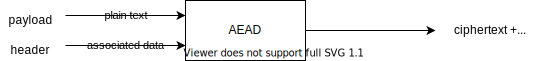
\includegraphics[width=\textwidth]{img/packet_enc.png}
    \caption{Payload encryption}
    \label{fig:payload_enc}
\end{figure}

\subsection{Header encryption}
Figure \ref{fig:header_enc} shows the process of header encryption.
The first step is to get \textit{sample} from encrypted payload.
In most cases a sample is 16 bytes long and it is taken starting from $4 - pn\_len$ byte of encrypted payload.
In the next step the sample is encrypted and its first 5 bytes are taken as mask.
At the end we perform XOR operation on predefined header fields and mask.
As a result we get header with some fields being encrypted.
Algorithm used to encrypt sample depends on negotiated cipher-suite.
For example, if payload is encrypted with AES\_128\_GCM then sample will be encrypted using AES\_128\_ECB.

\begin{figure}[h]
    \centering
    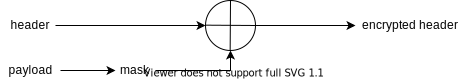
\includegraphics[width=\textwidth]{img/header_enc.png}
    \caption{Header encryption}
    \label{fig:header_enc}
\end{figure}

\subsection{Tests}
The test compares time needed to encrypt header and time needed to encrypt payload.
Payload encryption was performed with various data sizes (from 100 bytes to 1300 bytes).
Header length was constant and equal to 22 bytes. 
Encryption process was performed concurrently. 

\subsubsection{Environment}
Test environment:
\begin{itemize}
    \item processor: Intel(R) Core(TM) i5-9600K CPU @ 3.70GHz, 6 Cores, 9 MB Cache 
    \item memory: 16 GB RAM
    \item operating system: Linux 
    \item library: ring 0.16.20
    \item language: Rust
    \item cipher-suite: AES\_128\_GCM
\end{itemize}

\subsection{Results}

Figure \ref{fig:header_enc} shows header encryption time. 
The size of header was 22 bytes.
There were 100 samples. 
One sample was classified as mild outlier and marked with yellow color.
The rest was marked as clean samples.
The average is about 27.6 ns. 

\begin{figure}[h]
    \centering
    \includegraphics[width=\textwidth]{img/header_enc_result.png}
    \caption{Header encryption time}
    \label{fig:header_enc_result}
\end{figure}

Figure \ref{fig:header_payload_enc} presents time comparison between header and payload encryption process. 
Header size is constant and always equal to 22 bytes.
Payload size is from 100 to 1300 bytes.
We can see that payload encryption time is between 220 and 450 ns.
For 400, 800 and 1200 bytes we can observe shorter encryption time than for previous sizes.
This is probably because of concurrent execution of encryption process.
The data can be split across threads in a manner that allocates additional thread for 400, 800 and 1200 bytes.

\begin{figure}
    \centering
    \includegraphics[width=\textwidth]{img/header_payload_enc.png}
    \caption{Header vs payload time encryption}
    \label{fig:header_payload_enc}
\end{figure}

In summary, header encryption does not introduce a significant overhead for the entire packet encryption process.
